\documentclass[tikz,border=10pt]{standalone}
\usetikzlibrary{angles}
\begin{document}
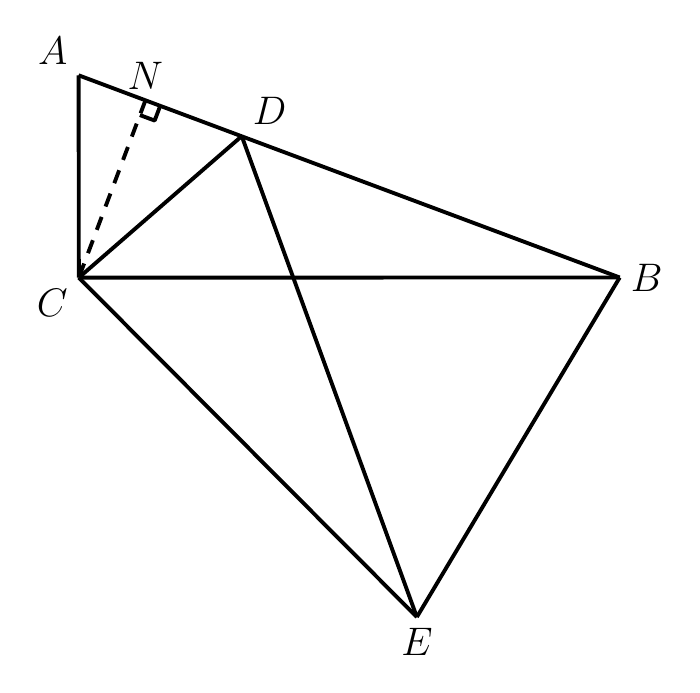
\begin{tikzpicture}[line width=1.4pt, line join=round]
\coordinate (A) at (-3.462,3.604);
\coordinate (B) at (3.410,1.036);
\coordinate (C) at (-3.459,1.034);
\coordinate (D) at (-1.390,2.831);
\coordinate (N) at (-2.613,3.286);








\coordinate (E) at (0.834,-3.276);


\draw (A) -- (N) -- (B);   
\draw (C) -- (B);          
\draw (A) -- (C);          
\draw (E) -- (D);          
\draw (D) -- (C);
\draw (E) -- (C);
\draw (B) -- (E);
\draw[dash pattern=on 5pt off 4pt] (N) -- (C);  


\pic[draw, angle radius=0.200cm] {right angle=C--N--B};


\node[above left]  at (A) {\fontsize{14.5}{17.4}\selectfont $A$};
\node[above]       at (N) {\fontsize{14.5}{17.4}\selectfont $N$};
\node[above right] at (D) {\fontsize{14.5}{17.4}\selectfont $D$};
\node[below left]  at (C) {\fontsize{14.5}{17.4}\selectfont $C$};
\node[right]       at (B) {\fontsize{14.5}{17.4}\selectfont $B$};
\node[below]       at (E) {\fontsize{14.5}{17.4}\selectfont $E$};
\end{tikzpicture}
\end{document}